\newpage

\subsection{A Cram\'{e}r-Lundberg process with a matrix exponential density} \label{e:MatExpCos}

In the following example, we study a \CL\ model with density of claims given by
\begin{align*}
f(x)=& u e^{-a x} 2 \cos ^{2}\left(\frac{\omega x+\phi}{2}\right)=u e^{-a x}(1+\cos (\omega x+\phi))=\\=& e^{-a x}(u+u \cos (\phi) \cos (\omega x)-u \sin (\phi) \sin (\omega x))
\end{align*}
where
\[u=\frac{a\left(a^{2}+\omega^{2}\right)}{a^{2}+\omega^{2}+a^{2} \cos (\phi)-a \omega \sin (\phi)}. \]
One can check that $\int f(x) d x=1$ with such value of $u$.

Assuming further that $a=1$, $\phi=2$, $\omega=20$, and that $\theta=1$, $q=1/10$, the Laplace exponent for this process is
$\kappa(s) = \frac{s \left(2.09898 s^3+5.29695 s^2+843.502 s+420.846\right)}{(s+1.) \left(s^2+2. s+401.\right)}$ and the scale function is
\begin{align*}
W_q(x)  &= 0.824723 e^{0.0881484 x} -0.348141 e^{-0.540677 x} \\
   &+e^{-1.0117 x} \cos (19.9957 x) ~\Big( -(0.000285494\, +0.0000804151 i) \sin (39.9914 x)\\
   &-(0.0000804151\, +0.000285494 i)+(-0.0000804151+0.000285494 i) \cos (39.9914 x) \Big)\\
   &+e^{-1.0117 x} \sin (19.9957 x) ~\Big( -(0.0000804151\, -0.000285494 i) \sin (39.9914 x) \\
   & +(0.000285494\, +0.0000804151 i) \cos (39.9914 x)-(0.000285494\, -0.0000804151 i) \Big).
\end{align*}

\begin{figure}[!h]
    \centering
    \begin{subfigure}[b]{0.8\textwidth}
        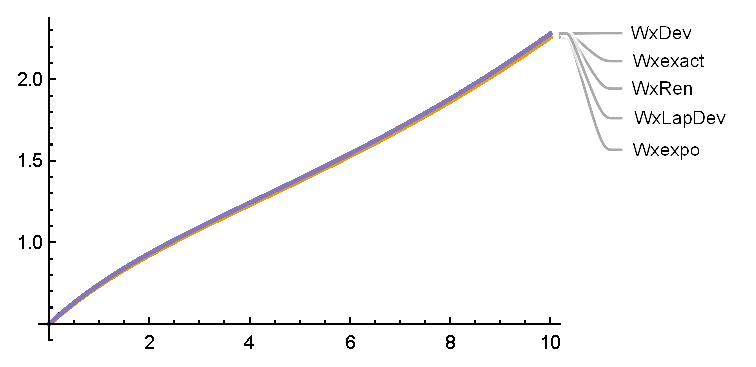
\includegraphics[width=\textwidth]{MatExpCosW}
        \caption{$W_q(x)$  (in black)}
        \label{fig:MatExpCosW}
    \end{subfigure}
    ~
    \\
    \begin{subfigure}[b]{0.8\textwidth}
        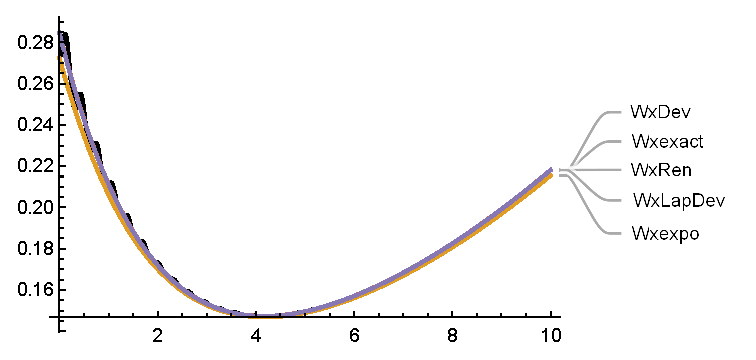
\includegraphics[width=\textwidth]{MatExpCosW1}
        \caption{$W'_q(x)$}
        \label{fig:MatExpCosW1}
    \end{subfigure}
    ~
    \\
    \begin{subfigure}[b]{0.8\textwidth}
        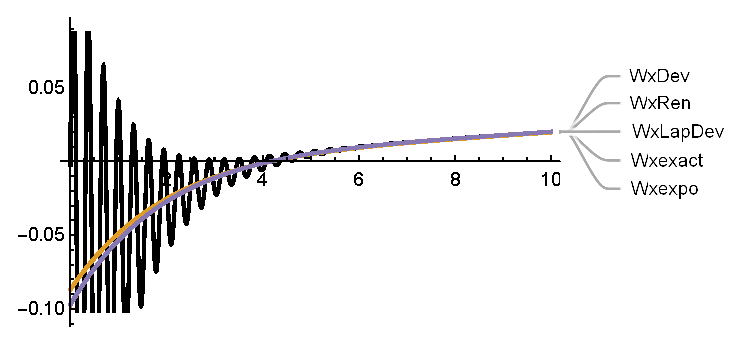
\includegraphics[width=\textwidth]{MatExpCosW2}
        \caption{$W''_q(x)$}
        \label{fig:MatExpCosW2}
    \end{subfigure}
    \caption{Plots of $W_q(x)$, $W'_q(x)$, and $W''_q(x)$ of the exact solution and the approximations for $f(x)= u e^{-a x} 2 \cos ^{2}\left(\frac{\omega x+\phi}{2}\right)$, $\th =1$, $q=\fr{1}{10}$.}\label{fig:MatExpCos}
\end{figure}


\begin{table}[!h]
\begin{tabular}{|l|l|l|l|l|}
\hline
       & \begin{tabular}[c]{@{}l@{}}Dominant   exponent \\ $\Phi_q$\end{tabular} & \begin{tabular}[c]{@{}l@{}}Percent   relative error\\ ($\Phi_q$)\end{tabular} & \begin{tabular}[c]{@{}l@{}}Optimal barrier\\ $b_{DeF}$\end{tabular} & \begin{tabular}[c]{@{}l@{}}Percent   relative error\\ ($b_{DeF}$)\end{tabular} \\ \hline
Exact  & 0.0881484                  & 0                                 & 4.38201              & 0                             \\ \hline
Expo   & 0.0878658                  & 0.32053                           & 4.42263              & 0.927122                      \\ \hline
Dev    & 0.0881484                  & 6.11743*10\textasciicircum{}-6    & 4.39745              & 0.352331                      \\ \hline
Renyi  & 0.0881481                  & 0.000314617                       & 4.39788              & 0.362284                      \\ \hline
LapDev & 0.0881449                  & 0.00395543                        & 4.3982               & 0.369586                      \\ \hline
\end{tabular}
\caption{Exact and approximate values of $\Phi_q$ and $b_{DeF}$ for $f(x)= u e^{-a x} 2 \cos ^{2}\left(\frac{\omega x+\phi}{2}\right)$, $\th =1$, $q=\fr{1}{10}$. The DeVylder approximation displayed the least percent relative error among the four approximations considered.}
\label{table:MatExpCos}
\end{table}
